\documentclass[12pt, titlepage]{article}

\usepackage{fullpage}
\usepackage[round]{natbib}
\usepackage{multirow}
\usepackage{booktabs}
\usepackage{tabularx}
\usepackage{graphicx}
\usepackage{float}
\usepackage{hyperref}
\hypersetup{
    colorlinks,
    citecolor=blue,
    filecolor=black,
    linkcolor=red,
    urlcolor=blue
}

%% Comments

\usepackage{color}

\newif\ifcomments\commentstrue %displays comments
%\newif\ifcomments\commentsfalse %so that comments do not display

\ifcomments
\newcommand{\authornote}[3]{\textcolor{#1}{[#3 ---#2]}}
\newcommand{\todo}[1]{\textcolor{red}{[TODO: #1]}}
\else
\newcommand{\authornote}[3]{}
\newcommand{\todo}[1]{}
\fi

\newcommand{\wss}[1]{\authornote{blue}{SS}{#1}} 
\newcommand{\plt}[1]{\authornote{magenta}{TPLT}{#1}} %For explanation of the template
\newcommand{\an}[1]{\authornote{cyan}{Author}{#1}}

%% Common Parts

\newcommand{\progname}{ProgName} % PUT YOUR PROGRAM NAME HERE
\newcommand{\authname}{Team \#, Team Name
\\ Student 1 name
\\ Student 2 name
\\ Student 3 name
\\ Student 4 name} % AUTHOR NAMES                  

\usepackage{hyperref}
    \hypersetup{colorlinks=true, linkcolor=blue, citecolor=blue, filecolor=blue,
                urlcolor=blue, unicode=false}
    \urlstyle{same}
                                


\newcounter{acnum}
\newcommand{\actheacnum}{AC\theacnum}
\newcommand{\acref}[1]{AC\ref{#1}}

\newcounter{ucnum}
\newcommand{\uctheucnum}{UC\theucnum}
\newcommand{\uref}[1]{UC\ref{#1}}

\newcounter{mnum}
\newcommand{\mthemnum}{M\themnum}
\newcommand{\mref}[1]{M\ref{#1}}

\begin{document}

\title{Module Guide for \progname{}} 
\author{\authname}
\date{\today}

\maketitle

\pagenumbering{roman}

\section{Revision History}

\begin{tabularx}{\textwidth}{p{3cm}p{2cm}X}
\toprule {\bf Date} & {\bf Version} & {\bf Notes}\\
\midrule
2025-03-21 & 1.0 & Initial Release\\
\bottomrule
\end{tabularx}

\newpage

\section{Reference Material}

This section records information for easy reference.

\subsection{Abbreviations and Acronyms}

\renewcommand{\arraystretch}{1.2}
\begin{tabular}{p{0.4\linewidth}  p{0.6\linewidth}}
  \toprule		
  \textbf{symbol} & \textbf{description}\\
  \midrule 
  AC & Anticipated Change\\
  BRIEF & Binary Robust Independent Elementary Features\\
  DAG & Directed Acyclic Graph \\
  FAST & Features from Accelerated Segment Test\\
  IFCS & Image Feature Correspondence Software \\
  M & Module \\
  MG & Module Guide \\
  ORB & Oriented Fast and Rotated Brief\\
  OS & Operating System \\
  R & Requirement\\
  SC & Scientific Computing \\
  SRS & Software Requirements Specification\\
  \progname & Program to identify and retrive regions of interest within the scene of camera imagery\\

  UC & Unlikely Change \\
  \bottomrule
\end{tabular}\\

\newpage

\tableofcontents

\listoftables

\listoffigures

\newpage

\pagenumbering{arabic}

\section{Introduction}

Decomposing a system into modules is a commonly accepted approach to developing
software.  A module is a work assignment for a programmer or programming
team~\citep{ParnasEtAl1984}.  We advocate a decomposition
based on the principle of information hiding~\citep{Parnas1972a}.  This
principle supports design for change, because the ``secrets'' that each module
hides represent likely future changes.  Design for change is valuable in SC,
where modifications are frequent, especially during initial development as the
solution space is explored.  

Our design follows the rules layed out by \citet{ParnasEtAl1984}, as follows:
\begin{itemize}
\item System details that are likely to change independently should be the
  secrets of separate modules.
\item Each data structure is implemented in only one module.
\item Any other program that requires information stored in a module's data
  structures must obtain it by calling access programs belonging to that module.
\end{itemize}

After completing the first stage of the design, the Software Requirements
Specification (SRS), the Module Guide (MG) is developed~\citep{ParnasEtAl1984}. The MG
specifies the modular structure of the system and is intended to allow both
designers and maintainers to easily identify the parts of the software.  The
potential readers of this document are as follows:

\begin{itemize}
\item New project members: This document can be a guide for a new project member
  to easily understand the overall structure and quickly find the
  relevant modules they are searching for.
\item Maintainers: The hierarchical structure of the module guide improves the
  maintainers' understanding when they need to make changes to the system. It is
  important for a maintainer to update the relevant sections of the document
  after changes have been made.
\item Designers: Once the module guide has been written, it can be used to
  check for consistency, feasibility, and flexibility. Designers can verify the
  system in various ways, such as consistency among modules, feasibility of the
  decomposition, and flexibility of the design.
\end{itemize}

The rest of the document is organized as follows. Section
\ref{SecChange} lists the anticipated and unlikely changes of the software
requirements. Section \ref{SecMH} summarizes the module decomposition that
was constructed according to the likely changes. Section \ref{SecConnection}
specifies the connections between the software requirements and the
modules. Section \ref{SecMD} gives a detailed description of the
modules. Section \ref{SecTM} includes two traceability matrices. One checks
the completeness of the design against the requirements provided in the SRS. The
other shows the relation between anticipated changes and the modules. Section
\ref{SecUse} describes the use relation between modules.

\section{Anticipated and Unlikely Changes} \label{SecChange}

This section lists possible changes to the system. According to the likeliness
of the change, the possible changes are classified into two
categories. Anticipated changes are listed in Section \ref{SecAchange}, and
unlikely changes are listed in Section \ref{SecUchange}.

\subsection{Anticipated Changes} \label{SecAchange}

Anticipated changes are the source of the information that is to be hidden
inside the modules. Ideally, changing one of the anticipated changes will only
require changing the one module that hides the associated decision. The approach
adapted here is called design for
change.

\begin{description}
\item[\refstepcounter{acnum} \actheacnum \label{acHardware}:] The specific
  hardware on which the software is running.
\item[\refstepcounter{acnum} \actheacnum \label{acInput}:] The format of the
  initial input data.
\item[\refstepcounter{acnum} \actheacnum \label{acInConstrain}:] The constraints 
on the input parameters.
\item[\refstepcounter{acnum} \actheacnum \label{acOutput}:] The format of the 
output data.
\item[\refstepcounter{acnum} \actheacnum \label{acOutConstrain}:] The constraints 
on the output results.
\item[\refstepcounter{acnum} \actheacnum \label{acNoise}:] The algorithm used to 
reduce noise within the imagery.
\item[\refstepcounter{acnum} \actheacnum \label{acKP}:] The algorithm used to 
identify keypoints in an image.
\item[\refstepcounter{acnum} \actheacnum \label{acFD}:] The algorithm used to 
define features within an image.
\item[\refstepcounter{acnum} \actheacnum \label{acFM}:] The algorithm used to 
compare features between images.
\item[\refstepcounter{acnum} \actheacnum \label{acMatches}:] The implementation 
of the data structure used to hold identified feature matches.
\item[\refstepcounter{acnum} \actheacnum \label{acRelation}:] The relationships 
between what methods of feature identification, description, and comparison are 
compatible with each other.
\item[\refstepcounter{acnum} \actheacnum \label{acVisualize}:] The user wants 
to visualize the outputs of a given processing operation.
\item[\refstepcounter{acnum} \actheacnum \label{acSaveImage}:] The user wants 
to save a snapshot of the output from any given processing operation.

\end{description}

\subsection{Unlikely Changes} \label{SecUchange}

The module design should be as general as possible. However, a general system is
more complex. Sometimes this complexity is not necessary. Fixing some design
decisions at the system architecture stage can simplify the software design. If
these decision should later need to be changed, then many parts of the design
will potentially need to be modified. Hence, it is not intended that these
decisions will be changed.

\begin{description}
\item[\refstepcounter{ucnum} \uctheucnum \label{ucIO}:] Input/Output devices
  (Input: File and/or Keyboard, Output: File, Memory, and/or Screen).
\item[\refstepcounter{ucnum} \uctheucnum \label{ucGoal}:]  The goal of the system 
is to identify and compare features identified within different images.
\item[\refstepcounter{ucnum} \uctheucnum \label{ucDetectMethod}:]  The methods of 
feature detection can be executed using parameters defined in the input parameters 
module.
\item[\refstepcounter{ucnum} \uctheucnum \label{ucMatchMethod}:]  The methods used 
to compare features can be executed using parameters defined in the input parameters 
module.
\item[\refstepcounter{ucnum} \uctheucnum \label{ucConfig}:]  The user interface is 
changed from a .config file and command line arguments to a novel user GUI.
  
\end{description}

\section{Module Hierarchy} \label{SecMH}

This section provides an overview of the module design. Modules are summarized
in a hierarchy decomposed by secrets in Table \ref{TblMH}. The modules listed
below, which are leaves in the hierarchy tree, are the modules that will
actually be implemented. Modules are numbered by \textbf{M} followed by a number.
\begin{description}
\item [\refstepcounter{mnum} \mthemnum \label{mHH}:] Hardware Hiding Module
\item [\refstepcounter{mnum} \mthemnum \label{mC}:] Control Module
\item [\refstepcounter{mnum} \mthemnum \label{mIF}:] Input Format Module
\item [\refstepcounter{mnum} \mthemnum \label{mSP}:] Specification Parameters Module
\item [\refstepcounter{mnum} \mthemnum \label{mOF}:] Output Format Module
\item [\refstepcounter{mnum} \mthemnum \label{mOV}:] Output Verification Module
\item [\refstepcounter{mnum} \mthemnum \label{mIS}:] Image Smoothing Module
\item [\refstepcounter{mnum} \mthemnum \label{mKD}:] Keypoint Detection Module
\item [\refstepcounter{mnum} \mthemnum \label{mFD}:] Feature Descriptor Module
\item [\refstepcounter{mnum} \mthemnum \label{mFM}:] Feature Matching Module
\item [\refstepcounter{mnum} \mthemnum \label{mIP}:] Image Plot Module
\item [\refstepcounter{mnum} \mthemnum \label{mOpenCV}:] OpenCV Library
\end{description}


\begin{table}[h!]
\centering
\begin{tabular}{p{0.3\textwidth} p{0.6\textwidth}}
\toprule
\textbf{Level 1} & \textbf{Level 2}\\
\midrule

{Hardware-Hiding Module} & ~ \\
\midrule

\multirow{10}{0.3\textwidth}{Behaviour-Hiding Module} & \mref{mC} Control Module\\ 
& \mref{mIF} Input Format Module\\
& \mref{mSP} Specification Parameters Module\\
& \mref{mOF} Output Format Module\\
& \mref{mOV} Output Verification Module\\
& \mref{mIS} Image Smoothing Module\\
& \mref{mKD} Keypoint Detection Module\\ 
& \mref{mFD} Feature Descriptor Module\\
& \mref{mFM} Feature Matching Module\\
& \mref{mIP} Image Plot Module\\
\midrule

\multirow{1}{0.3\textwidth}{Software Decision Module} & \mref{mOpenCV} OpenCV Library\\

\bottomrule

\end{tabular}
\caption{Module Hierarchy}
\label{TblMH}
\end{table}

\section{Connection Between Requirements and Design} \label{SecConnection}

The design of the system is intended to satisfy the requirements developed in
the SRS. In this stage, the system is decomposed into modules. The connection
between requirements and modules is listed in Table~\ref{TblRT}.

\section{Module Decomposition} \label{SecMD}

Modules are decomposed according to the principle of ``information hiding''
proposed by \citet{ParnasEtAl1984}. The \emph{Secrets} field in a module
decomposition is a brief statement of the design decision hidden by the
module. The \emph{Services} field specifies \emph{what} the module will do
without documenting \emph{how} to do it. For each module, a suggestion for the
implementing software is given under the \emph{Implemented By} title. If the
entry is \emph{OS}, this means that the module is provided by the operating
system or by standard programming language libraries.  \emph{IFCS} means the
module will be implemented by the \progname{} software.

Only the leaf modules in the hierarchy have to be implemented. If a dash
(\emph{--}) is shown, this means that the module is not a leaf and will not have
to be implemented.

\subsection{Hardware Hiding Modules (\mref{mHH})}

\begin{description}
\item[Secrets:]The data structure and algorithm used to implement the virtual
  hardware.
\item[Services:]Serves as a virtual hardware used by the rest of the
  system. This module provides the interface between the hardware and the
  software. So, the system can use it to display outputs or to accept inputs.
\item[Implemented By:] OS
\end{description}

\subsection{Behaviour-Hiding Module}

\begin{description}
\item[Secrets:]The contents of the required behaviours.
\item[Services:]Includes programs that provide externally visible behaviour of
  the system as specified in the software requirements specification (SRS)
  documents. This module serves as a communication layer between the
  hardware-hiding module and the software decision module. The programs in this
  module will need to change if there are changes in the SRS.
\item[Implemented By:] --
\end{description}

\subsubsection{Control Module (\mref{mC})}

\begin{description}
\item[Secrets:]The procedure to run the program.
\item[Services:]Oversees execution of the overall program.
\item[Implemented By:] IFCS
\item[Type of Module:] Abstract Object
\end{description}

\subsubsection{Input Format Module (\mref{mIF})}
\begin{description}
\item[Secrets:]The format and structure of the input data.
\item[Services:]Converts the input data into the data structure used by the
  input parameters module.
\item[Implemented By:] IFCS
\item[Type of Module:] Abstract Data Type
\end{description}

\subsubsection{Specification Parameters Module (\mref{mSP})}

\begin{description}
\item[Secrets:] The default values and software limits for constraints on input 
variables.
\item[Services:]Read access for the input checks against the parameters in 
\mref{mIF}.
\item[Implemented By:] IFCS
\item[Type of Module:] Record
\end{description}

\subsubsection{Output Format Module (\mref{mOF})}

\begin{description}
\item[Secrets:]The format of the output data and the structure in which it is contained.
\item[Services:]Outputs the results of the matched features, including the source image and 
feature identifiers.
\item[Implemented By:] IFCS
\item[Type of Module:] Abstract Data Type
\end{description}


\subsubsection{Output Verification Module (\mref{mOV})}
\begin{description}
\item[Secrets:]Contains the algorithms used to check uniqueness of feature matches and their 
identifiers.
\item[Services:]Reviews the set of matches image features and flags any that are repeated 
or share the same point of origin.
\item[Implemented By:] IFCS
\item[Type of Module:] Abstract Data Type
\end{description}


\subsubsection{Image Smoothing Module (\mref{mIS})}
\begin{description}
\item[Secrets:]The Kernel parameters used to smooth the image.
\item[Services:]Defines the smoothing kernel using the parameters in the Input 
Format module.
\item[Implemented By:] IFCS
\item[Type of Module:] Abstract Data Type
\end{description}


\subsubsection{Keypoint Detection Module (\mref{mKD})}
\begin{description}
\item[Secrets:]The methods used to define features within images.
\item[Services:]Defines the available methods used to detect features using the 
parameters in the Input Format module.
\item[Implemented By:] IFCS
\item[Type of Module:] Abstract Data Type
\end{description}

\subsubsection{Feature Descriptor Module (\mref{mFD})}

\begin{description}
\item[Secrets:]The methods of defining features within images.
\item[Services:]Defines the available methods used to describe features using the parameters 
in the Input Format module.
\item[Implemented By:] IFCS
\item[Type of Module:] Abstract Data Type
\end{description}

\subsubsection{Feature Matching Module (\mref{mFM})}
\begin{description}
\item[Secrets:]The methods used to compare features within images.
\item[Services:]Defines the available methods used to compare image features using the 
parameters in the Input Format module.
\item[Implemented By:] IFCS
\item[Type of Module:] Abstract Data Type
\end{description}


\subsubsection{Image Plot Module (\mref{mIP})}
\begin{description}
\item[Secrets:]The methods used to generate  new images using identified image attributes.
\item[Services:]Defines the available methods used to generate and manipulate a new image. This may encrouch upon
\item[Implemented By:] IFCS
\item[Type of Module:] Abstract Data Type
\end{description}

\subsection{Software Decision Module}

\subsubsection{OpenCV Library (\mref{mOpenCV})}
\begin{description}
\item[Secrets:] The data structures and algorithms used to manipulate imagery data.
\item[Services:] Provides methods to import, manipulate, and export imagery data.
\item[Implemented By:] OpenCV library
\end{description}

\section{Traceability Matrix} \label{SecTM}

This section shows two traceability matrices: between the modules and the
requirements and between the modules and the anticipated changes.

% the table should use mref, the requirements should be named, use something
% like fref
\begin{table}[H]
\centering
\begin{tabular}{p{0.2\textwidth} p{0.6\textwidth}}
\toprule
\textbf{Req.} & \textbf{Modules}\\
\midrule
R1 & \mref{mHH}, \mref{mIF}\\
R2 & \mref{mHH}, \mref{mIF}\\
R3 & \mref{mHH}, \mref{mIF}\\
R4 & \mref{mHH}, \mref{mIF}\\
R5 & \mref{mSP}\\
R6 & \mref{mKD}\\
R7 & \mref{mFD}\\
R8 & \mref{mFM}\\
R9 & \mref{mIS}\\
R10 & \mref{mC}, \mref{mKD}\\
R11 & \mref{mC}, \mref{mFD}\\
R12 & \mref{mC}, \mref{mFM}\\
R13 & \mref{mOV}\\
R14 & \mref{mOF}\\
R15 & \mref{mOF}\\
\bottomrule
\end{tabular}
\caption{Trace Between Requirements and Modules}
\label{TblRT}
\end{table}

\begin{table}[H]
\centering
\begin{tabular}{p{0.2\textwidth} p{0.6\textwidth}}
\toprule
\textbf{AC} & \textbf{Modules}\\
\midrule
\acref{acHardware} & \mref{mHH}\\
\acref{acInput} & \mref{mIF}\\
\acref{acInConstrain} & \mref{mSP}\\
\acref{acOutput} & \mref{mOF}\\
\acref{acOutConstrain} & \mref{mOV}\\
\acref{acNoise} & \mref{mIS}\\
\acref{acKP} & \mref{mKD}\\
\acref{acFD} & \mref{mFD}\\
\acref{acFM} & \mref{mFM}\\
\acref{acMatches} & \mref{mOpenCV}\\
\acref{acRelation} & \mref{mC}\\
\acref{acVisualize} & \mref{mIP}\\
\acref{acSaveImage} & \mref{mIP}\\
\bottomrule
\end{tabular}
\caption{Trace Between Anticipated Changes and Modules}
\label{TblACT}
\end{table}

\section{Use Hierarchy Between Modules} \label{SecUse}

In this section, the uses hierarchy between modules is
provided. \citet{Parnas1978} said of two programs A and B that A {\em uses} B if
correct execution of B may be necessary for A to complete the task described in
its specification. That is, A {\em uses} B if there exist situations in which
the correct functioning of A depends upon the availability of a correct
implementation of B.  Figure \ref{FigUH} illustrates the use relation between
the modules. It can be seen that the graph is a directed acyclic graph
(DAG). Each level of the hierarchy offers a testable and usable subset of the
system, and modules in the higher level of the hierarchy are essentially simpler
because they use modules from the lower levels.

\begin{figure}[H]
\centering
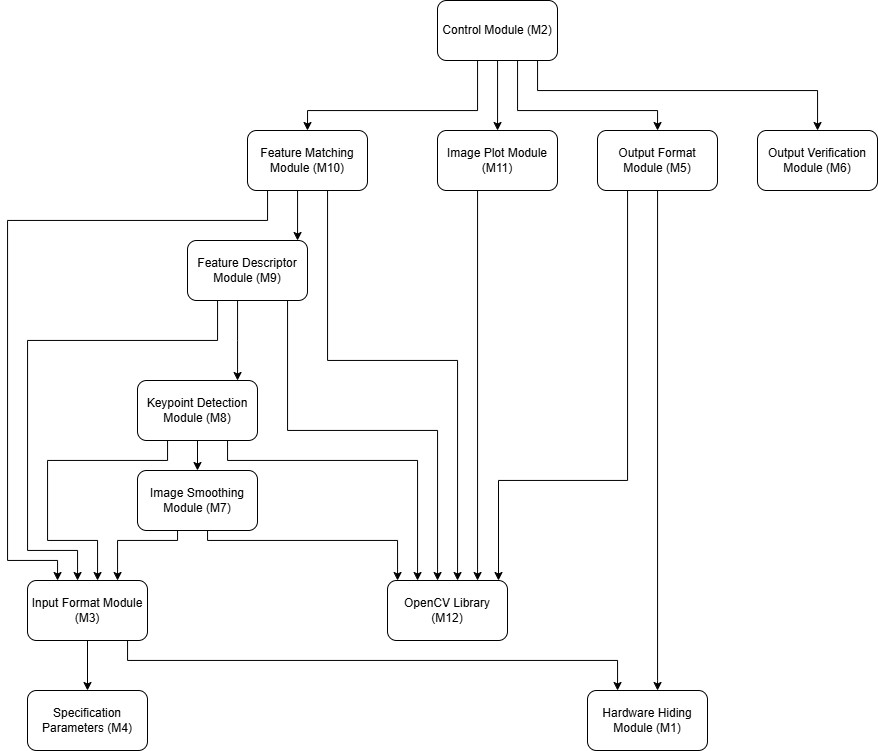
\includegraphics[width=0.7\textwidth]{UsesHierarchy.png}
\caption{Use hierarchy among modules}
\label{FigUH}
\end{figure}

\section{Timeline}
Table \ref{MG_Timeline} outlines the schedule of tasks that will be performed by members of the VnV team, as defined in 
the \href{https://github.com/KiranSingh15/CAS-741-Image-Correspondences/blob/main/docs/VnVPlan/VnVPlan.pdf}{VnV Plan}.

\begin{table}[H]
  \centering
  \renewcommand{\arraystretch}{1.3} % Increases row height for readability
  \begin{tabular}{|p{7cm}|c|c|}
  \hline
  \multicolumn{1}{|c|}{\textbf{Task}} & \textbf{V\&V Team Assignee} & \textbf{Due By} \\ \hline
  \raggedright Implement Software Decision Modules for Implementation Presentation & Author & March 24, 2025 \\ \hline
  \raggedright Implement Behaviour Hiding Modules for Implementation Presentation & Author & March 26, 2025 \\ \hline
  \raggedright Review Modules and Provide Feedback & Domain Expert & March 26, 2025 \\ \hline
  \raggedright Finalize modules for final documentation & Author & April 11, 2025 \\ \hline
  \end{tabular}
  \caption{Development Timeline of the Module Guide/Interface Specification}
  \label{MG_Timeline}
\end{table}
  
\bibliographystyle {plainnat}
\bibliography{../../../refs/References}

\newpage{}

\end{document}